%\documentclass[11pt]{article}
\documentclass[answers]{exam}

\usepackage{amsmath}
%\usepackage{extsizes}
\usepackage{amsmath,amssymb}
%\usepackage{omegavn,ocmrvn}
%\usepackage[utf8x]{inputenc}
\usepackage[utf8]{vietnam}
\DeclareUnicodeCharacter{00A0}{ }

\usepackage{longtable}
\usepackage{answers}
\usepackage{graphicx}
\usepackage{array}
\usepackage{pifont}
\usepackage{picinpar}
\usepackage{enumerate}
\usepackage[top=3.0cm, bottom=3.5cm, left=3.5cm, right=2.5cm] {geometry}
\usepackage{hyperref}


\newtheorem{bt}{Câu}
\newcommand{\RR}{\mathbb R}
\Newassociation{sol}{Solution}{ans}
\newtheorem{ex}{Câu}
\renewcommand{\solutionstyle}[1]{\textbf{ #1}.}
\newcommand{\m}[1]{
	\begin{bmatrix}
		#1
	\end{bmatrix}
}

\begin{document}
% \noindent
\begin{tabular*}
{\linewidth}{c>{\centering\hspace{0pt}} p{.7\textwidth}}
Trường ĐHKHTN, ĐHQGHN & {\bf Cao học 2020 - 2021 }
\tabularnewline
Khoa Toán - Cơ - Tin học \\ Lớp thầy Hà Phi & {\bf Bài Tập Numerics 4 PDEs. \\  No 1. Finite Difference Methods }
\tabularnewline
\rule{1in}{1pt}  \small  & \rule{2in}{1pt} %(Due date:)
\tabularnewline

%  \tabularnewline
%  &(Đề thi có 1 trang)
\end{tabular*}
%
%\Opensolutionfile{ans}[ans1]
\printanswers

\begin{bt}
a) Hãy tìm các công thức sai phân bậc cao hơn để xấp xỉ đạo hàm cấp 2 $f"(x)$ sử dụng công thức Taylor như trong tuần 2. \\
b) Hãy lập trình để đi tìm thêm ít nhất 3 công thức nữa và vẽ hình như trong Video tuần 2 (W2V6 High Order, phút 2.34). \\
\vskip .2cm
%
\textbf{
Trong các bài tập dưới đây chúng ta xét các phương trình sóng trong không gian 2 chiều (2D acoustic wave equation)
%
\begin{equation}\label{1}
p_{tt} = c^2(x,y) \ \left( p_{xx} + p_{yy} \right) + s(x,y,t), \quad (x,y,t) \in \Omega \times [0,T],
\end{equation}
%
cùng với các điều kiện ban đầu
%
\begin{align}
p(x, y, 0) = f_1(x, y), \ (x,y) \in \Omega, \\
p_t(x, y, 0) = f_2(x, y), \ (x,y) \in \Omega
\end{align}
%
và điều kiện biên
%
\begin{equation}\label{2}
p(x, y, t) = g(x, y, t), \ 	\quad (x,y,t) \in \partial \Omega \times [0,T],
\end{equation}
%
trong đó $c(x, y)$ là vận tốc sóng (wave velocity) và $\Omega \subset \RR^2$ là một miền bị chặn và $s(x,y,t)$ là hàm nguồn sóng (source). \\
%
Để thu được các phương pháp số chính xác hơn, thông thường các đạo hàm cấp 2 theo biến không gian sẽ được xấp xỉ bằng các công thức sai phân cấp cao hơn (sử dụng nhiều hơn 3 điểm) 
hãy đặt option 3 hoặc 5 như trong code của bài giảng. \\
%
Phương pháp số được gọi là hội tụ bậc $(p,q)$ nếu như ta có ước lượng sai số tuyệt đối 
%
\[
\underset{\Omega \times [0,T] }{\sup} | p_{exact}(x,y,t) - p_{approx}(x,y,t) | \leq C \left( \Delta t^p + \Delta x ^q + + \Delta y ^q \right).
\]
%
Hầu hết các sơ đồ FD để giải phương trình sóng âm là ổn định có điều kiện và chịu hạn chế về bước thời gian $\Delta t$. 
Thông thường chúng ta phân tích độ ổn định của phương pháp số bằng cách sử dụng phân tích độ ổn định Von Neumann.
Điều đáng nói là phân tích độ ổn định Von Neumann chỉ áp dụng cho trường hợp vận tốc không đổi. Mặc dù rất khó để áp dụng phương pháp phân tích von Neumann trực tiếp cho trường hợp không đồng nhất, ta có thể thay $c(x, y)$ bằng $c_{max}$, đó là giá trị lớn nhất của $c(x, y)$ trên miền $\Omega$.
}
\end{bt}

\begin{bt} (Bài toán biên $0$) \\
a) Hãy giải gần đúng phương trình sóng \eqref{1} trên miền $\Omega = [0,\pi] \times [0,\pi]$ với $t\in [0,1]$, và nghiệm chính xác có dạng 
$p(x, y, t) = \cos(t) \sin(x) \sin(y)$. Các điều kiện biên và điều kiện ban đầu được chọn sao cho nghiệm này thỏa mãn chúng. 
Vận tốc sóng là $c(x, y) = \sqrt{ 1 +  \left( \dfrac{x}{\pi} \right)^2 + \left( \dfrac{y}{\pi}\right)^2 }$, và nguồn sóng là
$s(x,y,t) = \left( 1 +  2 \left( \dfrac{x}{\pi} \right)^2 + 2 \left( \dfrac{y}{\pi} \right)^2 \right) \cos(t) \sin(x) \sin(y)$. \\
b) Hãy tìm bậc hội tụ $(p,q)$ trong hai trường hợp $op=3$ và $op=5$. \\
c) Thiết lập điều kiện CFL cho tính hội tụ của phương pháp để tìm mối liên hệ giữa bước thời gian và bước không gian. 
Để đơn giản lấy $\Delta x = \Delta y = 12,5$ m (lưới đều). 
Hãy điều chỉnh các bước thời gian và không gian để kiểm tra tính ổn định/hội tụ của phương pháp. 
\end{bt}

\begin{bt} (Bài toán biên khác $0$) \\
Trong bài tập này chúng ta thay đổi vận tốc sóng sao cho $c^2(x, y) = 1 + \sin^2(x) + \sin^2(y)$. Công thức nghiệm chính xác là 
$p(x, y, t) = e^{-t} \cos(x) \cos(y)$. 
Các điều kiện biên và điều kiện ban đầu được chọn sao cho nghiệm này thỏa mãn chúng. Hãy thực hiện lại các câu hỏi trong bài tập 2 ở trên. 
\end{bt}

\begin{bt}
Trong bài tập này chúng ta sẽ có một nguồn phát sóng tại 1 điểm  trong miền $[0, 5 \ km ] \times [0, 5 \ km]$ bao gồm 2 lớp, như trong Hình \ref{fig:fig1}. 
Hai lớp này đều là thuần nhất với vận tốc sóng tương ứng là $c_{upper} = 1500$ m/s và $c_{lower} = 3000$ m/s. 
Nguồn wavelet của Ricker tạo ra sóng được cho bởi
%
\[
s (x, y, t) = \delta (x - x_0, y - y_0) \left[ 1 - 2\pi^2 f_p^2 (t - dr)^2\right]  e^ {- \pi^2 f_p^2 (t - dr)^2},
\]
%
với $f_p = 10$ Hz là tần số chính (dominant frequency). Ở đây, $dr = 0,5 / f_p$ là độ trễ tạm thời được sử dụng để đảm bảo điều kiện ban đầu bằng không. \\
a) Hãy giải số bài toán này. Đối với tất cả các mô phỏng số, hãy sử dụng kích thước lưới đồng nhất $\Delta_x = \Delta_y = 12,5$ m. Để đơn giản, hãy xét điều kiện biên bằng không. Mặc dù vây, trong thực tế, cần có điều kiện phân lớp phù hợp. \\
b) Để thể hiện độ phân tán số, hãy vẽ đồ thị các biên độ của các trường sóng được lấy mẫu tại x = 2500 m trong thời gian t = 0,3 s, 0,65 s, 0,95 s và 1,15 s. \\
%
\begin{figure}[h!]
	\centering
	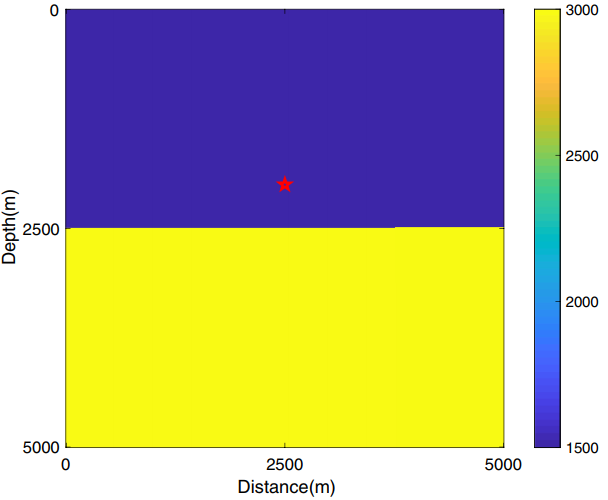
\includegraphics[scale = 0.7]{Fig1}
	\caption[]{Mô hình vận tốc bao gồm hai lớp đồng nhất với vận tốc âm không đổi 1500 m / s ở lớp trên, và vận tốc không đổi 3000 m / s ở lớp dưới. Ngôi sao màu đỏ cho biết nguồn nằm ở (2500 m, 2000 m).}
	\label{fig:fig1}
\end{figure}
\end{bt}

 \newpage 

\begin{bt}
Mô hình Marmousi, được thể hiện trong Hình \ref{fig:fig2}. Cùng một nguồn Ricker’s wavelet được sử dụng, với thời gian trễ hơi khác 
$dr = 0,3 / f_p$. Mô hình vận tốc được xác định trên lưới với khoảng cách đều h = 15 m, trên miền $\Omega$ là hình chữ nhật 
$[0, 10500 \ m] \times [0, 5250 \ m ]$. Hãy giải quyết các câu hỏi tương tự như trong bài tập 4: \\ 
a) Hãy giải số bài toán này. Đối với tất cả các mô phỏng số, hãy sử dụng kích thước lưới đồng nhất $\Delta_x = \Delta_y = 15$ m. Để đơn giản, hãy xét điều kiện biên bằng không. Mặc dù vây, trong thực tế, cần có điều kiện phân lớp phù hợp. \\
b) Để thể hiện độ phân tán số, hãy vẽ đồ thị các biên độ của các trường sóng được lấy mẫu tại x = 2500 m trong thời gian t = 0.9, 1.2, 1.5 s. \\
%
\begin{figure}[h!]
	\centering
	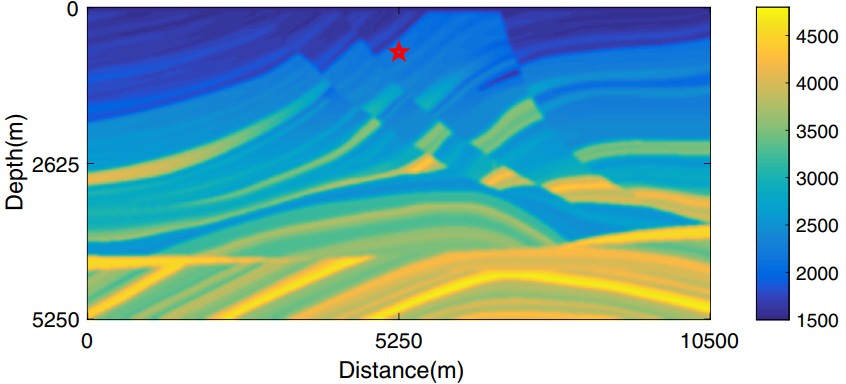
\includegraphics[scale = 0.7]{Fig2}
	\caption[]{Mô hình Marmousi được xác định trên miền hình chữ nhật $ 10500 \ m \ times 5250 \ m $. Vận tốc dao động từ $ 1500 m / s $ đến $ 4800 m / s $. Nguồn, ký hiệu là ngôi sao màu đỏ, nằm ở (5250 m, 750 m). }
	\label{fig:fig2}
\end{figure}
\end{bt}

\centerline{———————————Hết——————————}

%\vspace{1cm}
%\noindent{\bf Chú ý:} {\it Cán bộ coi thi không giải thích gì thêm}\\
%\vspace{0.4cm}
%\noindent{\bf Họ và tên học \sinh: \rule{3in}{.01pt} Lớp: \hrulefill}
%\Closesolutionfile{ans}
%\newpage
%\begin{center}
%{\LARGE{\bf ĐÁP ÁN}}
%\end{center}
%\begin{Solution}{1}
	\begin{figure}[h!]
		\centering
		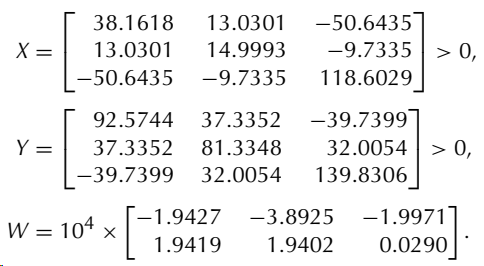
\includegraphics[width=0.7\linewidth]{Solution1/screenshot001}
		\caption[Exercise 1.2.5, Burden-Faires, 8ed.]{}
		\caption{}
		\label{fig:screenshot001}
	\end{figure}
\end{Solution}
 
   
\end{document}